\section{Synthèse du travail d'intégration continue}
\label{sec:synthese_ci}
L'amélioration du CI d'Alter-Frame et l'ajout de la composante sécurité a été la tâche principale de mon stage.

Un point sur le fonctionnement et la nomenclature de GitLab-CI\footnote{GitLab maintient une page de présentation de leur service CI plus complète \href{https://about.gitlab.com/2016/10/25/gitlab-workflow-an-overview/}{ici}.} : le script de contrôle du processus de CI est le \texttt{.gitlab-ci.yml}, ou le \texttt{.yml} pour faire court. Le comportement par défaut pour ce script est de définir une image Docker, avec la balise \texttt{image} (on aurait par exemple \texttt{image: openjdk:latest} pour aller chercher l'image openjdk sur le hub docker, et récupérer la version taguée "latest").

Cette image va être instanciée en un container au début de l'exécution du script, et ce dernier se déroulera dans l'environnement du container. Utiliser l'image openjdk par exemple donne accès à une JDK et permet donc d'appeler des fonctions telles que javac ou d'installer des utilitaires qui en dépendent tels que SonarQube. 

On appelle "runner" l'hôte sur lequel s'exécute l'image docker, et "job" chacune des fonctions en lesquelles le script peut être séparé. Eux-mêmes peuvent être regroupés en stages : les stages s'exécutent dans l'ordre dans lequel ils sont déclarés et si un stage échoue, le runner s'arrête. En revanche, l'ordre des jobs au sein d'un stage est à la discrétion du runner et ne peut pas être connu. 

La figure~\ref{fig:ci_flow} résume le fonctionnement de GitLab-CI. 

\begin{figure}
  \centering
  \caption{Résumé du processus de CI (\emph{build}, \emph{test} et \emph{deploy} sont les stages par défaut)}
  \label{fig:ci_process}
  \frame{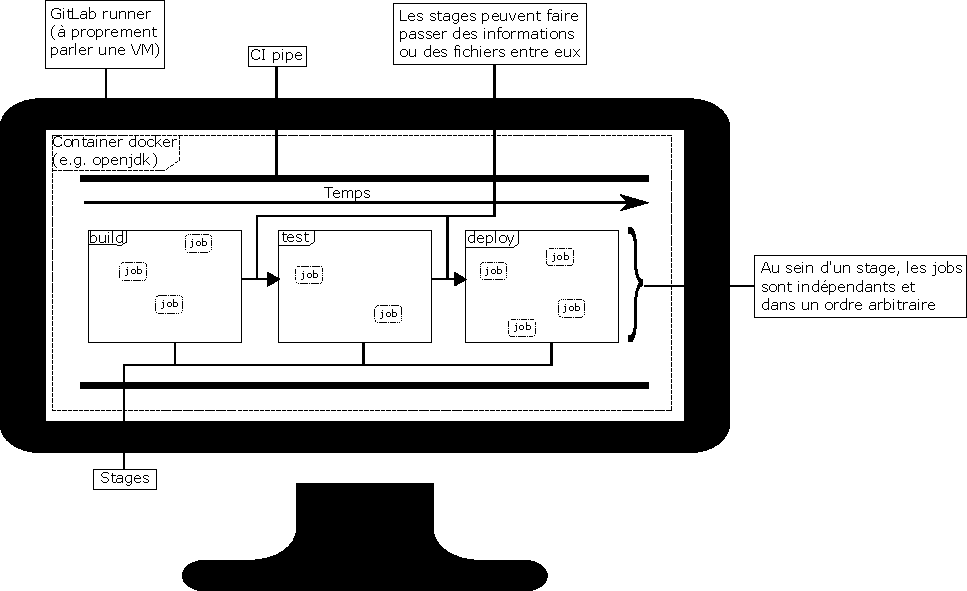
\includegraphics[width=\textwidth]{images/process_ci.pdf}}
\end{figure}

\subsection{Déployer automatiquement les applications web}
Mon intervention sur cette partie a été en commun avec un autre ingénieur d'Alter Frame. Nous devions faire en sorte de compiler les applications web en PHP, et générer à partir de là une image Docker contenant l'application\footnote{La documentation sur l'utilisation de \texttt{docker build} dans GitLab-CI : \url{https://docs.gitlab.com/ee/ci/docker/using_docker_build.html#using-docker-build}} et toute la configuration requise, puis  déployer cette image sur un serveur appartenant à Alter Frame.

Voilà pour la théorie. La pratique a été une succession d'approches différentes qui n'ont pas toujours été fructueuses, et beaucoup d'essai et échec permettant d'avancer petit à petit ; il faut savoir que la documentation de GitLab-CI sur le sujet\footnote{\url{https://docs.gitlab.com/ce/ci/docker/using_docker_build.html}} n'est pas parfaitement complète et fait la supposition que l'utilisateur possède une bonne connaissance de Docker.

La première approche fut d'exécuter le runner en mode shell plutôt que Docker. C'est la méthode la plus facile mais aussi celle qui s'éloigne le plus du comportement par défaut et qui fait perdre la grande flexibilité qu'offre le fonctionnement par image Docker : les différents outils doivent être définitivement installés sur le serveur qui héberge les runners. 

En plus de ce défaut, cette méthode est discutable d'un point de vue sécurité car elle exige que l'utilisateur qui exécute le script ait des privilèges administrateur, donc indirectement toute personne qui intervient sur les scripts .yml\footnote{Un article sur la sécurité du groupe Docker : \url{https://www.andreas-jung.com/contents/on-docker-security-docker-group-considered-harmful}}.

Au final et malgré ses points négatifs, cette méthode nous a permis d'arriver à nos fins, mais nous ne l'avons pas retenue, pour partie pour les raisons exposées plus haut et pour partie pour des raisons propres à la compilation de l'application en PHP qui bloquaient l'ingénieur avec lequel j'ai travaillé. 

Deuxième approche, plus en accord avec la philosophie de GitLab-CI : utiliser docker-in-docker (dind). L'idée est simple et la mise en oeuvre plus complexe (pour changer). Il s'agit de fournir au runner une image disposant des utilitaires nécessaires pour construire une image docker, et finalement de réaliser le même processus qu'en mode shell, mais dans le contexte isolé du container docker parent.

Les inconvénients de la méthode shell disparaissent : plus besoin d'installer en dur sur le serveur des utilitaires qui sont spécifiques à un projet (le serveur héberge plusieurs runners qui se répartissent tous les projets d'Alter Frame selon les besoins) ; plus besoin non plus d'avoir des privilièges administrateur sur le serveur.

Bien entendu cette méthode aussi avait un coût. Tout d'abord, GitLab-CI met en place des protections pour éviter que tout développeur puisse, par défaut, avoir accès à ces fonctionnalités et il faut donc une étape de configuration supplémentaire au niveau des runners pour utiliser dind.

Ensuite, déployer et configurer une application est un procédé lourd qui peut impliquer l'installation de dépendances. En réalisant cela dans un container, deux cas de figure se présentent :
\begin{itemize}[label=$\bullet$]
\item soit on utilise une image générique proposant l'outil de base (e.g. openjdk:latest pour un projet Java) et on installe dans le .yml les différentes dépendance. Ce n'est pas compliqué de mise en oeuvre, mais chaque exécution du script sera longue, et la lenteur est vite limitante dans le domaine de l'intégration continue (le développeur n'a pas toujours le temps d'attendre qu'un procédé long se termine) ;
\item soit on crée une image personnalisée qui embarque déjà les dépendances requises, cela accélère le processus de CI mais rajoute du travail en amont avec la création et la configuration de l'image, ainsi que son stockage sur un registre Docker. De plus, le processus perd en transparence car la configuration de l'environnement devient cachée au développeur qui ne voit que le nom de l'image utilisée. Bien sûr, cela peut aussi être vu comme un avantage car le .yml s'en trouve d'autant allégé, et ne contient au final plus que l'essentiel du point de vue intégration et déploiement. 
\end{itemize}
% TODO : mettre le listing du dockerfile que j'ai créé

C'est la deuxième approche que j'ai conservée, mais non sans avoir testé la première au préalable. Avoir la configuration directement dans le .yml était source de complexité (appeler un .sh à l'intérieur du .yml pour extenaliser de gros blocs de code) et de bugs (de petits changements pouvaient entraîner des résultats inattendus, surtout compte tenu du fait que nous étions plusieurs à intervenir sur le .yml).

% TODO : parler un peu de ce que j'ai dû faire dans le dockerfile comme config

Au final, cette méthode a tenu ses promesses : nous nous retrouvions avec une configuration sauvegardée à part, facile et rapide à importer, et qui comportait toutes les dépendances requises pour le projet. De plus un runner avait été spécialement configuré pour permettre l'utilisation de dind, restreinte par défaut, et générer l'image qui encapsulait l'appli web développée par Alter Frame devenait possible.

\subsection{Intégrer ZAP et les analyses de sécurité}
ZAP a pour lui d'intégrer par défaut les cas d'usage qui m'importaient, à savoir de pouvoir être utilisé en mode ligne de commade et/ou contrôlé par une API sans interaction avec l'utilisateur au moment de l'exécution.

De ces deux solutions, c'est celle de l'API qui est la plus complète : ZAP en ligne de commande propose quelques options
% TODO : mettre un lien vers le listing de ZAP de la partie d'avant
mais qui sont vite limitées : se connecter à un site web, lancer certaines des commandes de base de l'application comme le crawler ou le scan actif, et générer un fichier de résultats. Le scan actif de ZAP est tout de même assez intéressant pour que cette méthode soit pertinente, mais les options proposées par les APIs sont bien plus foisonnantes.

Néanmoins, la solution de l'API rajoute une contrainte : en plus de ZAP, il faut que l'environnement de CI dispose du langage de l'API. Les deux APIs principales maintenues par la communauté de développeurs ``officiels'' de ZAP sont celles en Java et en Python. J'ai retenu l'utilisation de Python d'une part car ce langage est concis et se prête très bien à l'écriture de courts scripts, d'autre part pour avoir l'occasion de m'en servir et développer des compétences qui me seraient utiles plus tard dans mon parcours professionnel.
% TODO : lien vers la partie "avenir" pour dire que je vais me servir de python

Plutôt que de rajouter encore un élément à l'image Docker créée spécialement au point précédent, j'ai préféré utiliser une fonctionnalité très intéressante de GitLab-CI, celle de pouvoir spécifier une image différente pour chaque job. Elle rajoute en verbosité au script car l'image doit donc être spécifiée pour chaque job sans exception (impossible d'en utiliser une par défaut et de ne la remplacer que pour le job de l'analyse ZAP), mais elle évite de surcharger l'image Docker utilisée pour le déploiement. Qui plus est, cette image de déploiement est spécifique à chaque projet et doit donc être réécrire, alors que le script commendant l'exécution de ZAP peut être générique (exception faite de l'URL cible). Inclure l'image à utiliser à ce script renforce cette autonomie, le bloc de code peut littéralement être copié collé d'un projet à l'autre et fonctionner (encore une fois sous réserve de changer l'URL à attaquer).
%TODO : inclure le snippet de ZAP

\subsection{Méthodologie}
\subsection{Travail effectué}
